\chapter{Исследовательская часть}
В текущем разделе будут представлены примеры работы разработанного программного обеспечения, постановка эксперимента и сравнительный анализ реализованных алгоритмов.

\section{Пример работы программного обеспечения}

На рисунке \ref{fig:prog_exmpl} представлен результат работы программы.
На вход программы подаются две матрицы размерностей 3 на 4 и 4 на 3 соответственно.
Первая матрица -- [[1, 2, 3, 4], [5, 6, 7, 8], [9, 1, 2, 3]], вторая матрица -- [[6, 7, 9], [-1, -3, 4], [3, 7, 9], [17, -5, 6]].
В результате выполнения программа выводит матрицу, полученную умножением двух введенных пользователем матриц различными алгоритмами (стандартный, Винограда, оптимизированный Винограда).

\begin{figure}[h!]
	
	\centering{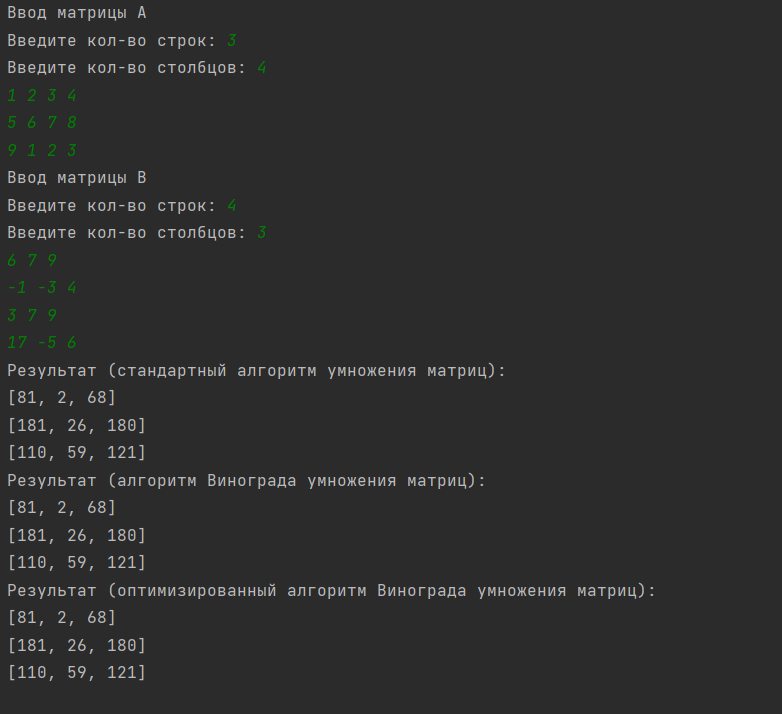
\includegraphics[scale=1]{inc/prog_exmpl.PNG}}
	
	\caption{Пример работы программы}
	
	\label{fig:prog_exmpl}
	
\end{figure}

\clearpage

\section{Технические характеристики}

Технические характеристики устройства, на котором выполнялось тестирование:

\begin{itemize}
	\item операционная система: Windows 10~\cite{windows10};
	\item оперативная память: 16 Гб;
	\item процессор: Intel® Core™ i5 10300H 2.5 ГГц.
\end{itemize}

Во время тестирования ноутбук был включен в сеть питания и нагружен только встроенными приложениями окружения и системой тестирования.

\section{Время выполнения реализаций алгоритмов}

Замеры процессорного времени реализованных алгоритмов сортировки (гномья сортировка, поразрядная сортировка, сортировка выбором) проводились с помощью функции process\_time() из библиотеки time языка Python. 

Функция process\_time() возвращает время в секундах (сумму системного и пользовательского процессорного времени).

Замеры времени для каждой четной размерности входных матриц (от 100 x 100 до 500 x 500 с шагом 100) и нечетной (от 101 x 101 до 501 x 501 с шагом 100) проводились 10 раз для всех трех реализованных алгоритмов умножения матриц. В качестве результата бралось среднее время работы алгоритма на каждой длине массива.


На рисунке \ref{fig:fig1} представлено сравнение процессорного времени работы реализаций алгоритмов умножения матриц на матрицах четной размерности (n * n).

На графике видно, что оптимизированный алгоритм Винограда является самым эффективным по времени среди реализованных алгоритмов и его преимущество растет с увеличением размера матрицы, на втором месте по эффективности -- алгоритм Винограда в классической реализации, самый неэффективный по времени -- стандартный алгоритм умножения матриц, но он практически не уступает по времени алгоритму Винограда без оптимизации.
\\
\\
\\
\\
\\
\\
\\
\\

\begin{figure}[h!]
	
	\centering{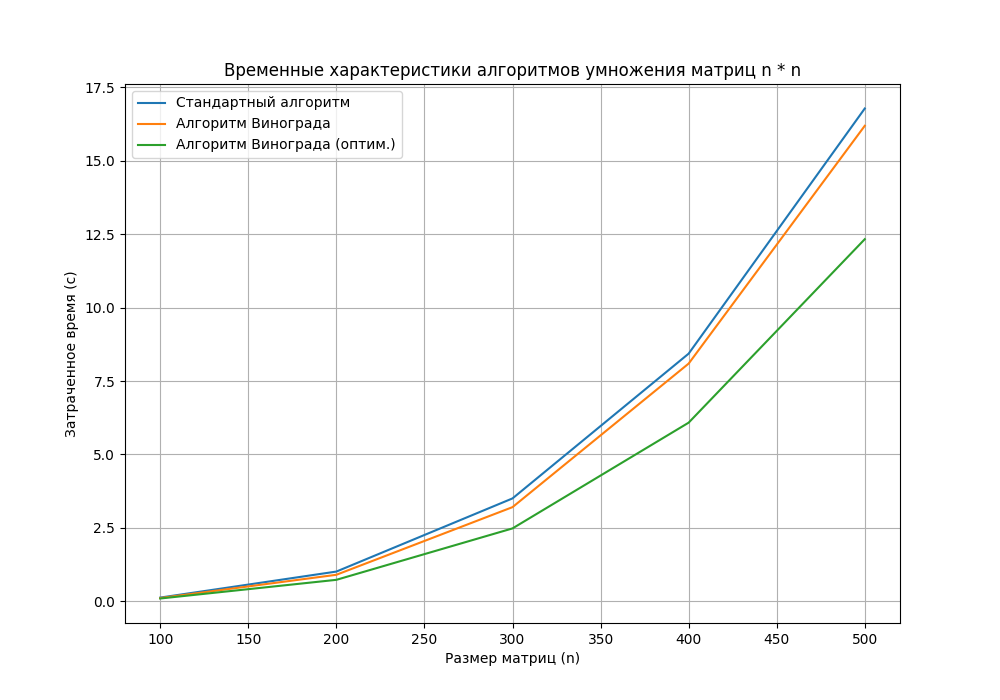
\includegraphics[scale=0.7]{inc/Figure_2.png}}
	
	\caption{Сравнение процессорного времени работы реализаций алгоритмов умножения матриц на квадратных матрицах четной размерности (n * n)}
	
	\label{fig:fig1}
	
\end{figure}

\clearpage
На рисунке \ref{fig:fig2} представлено сравнение процессорного времени работы реализаций алгоритмов умножения матриц на матрицах нечетной размерности (n + 1) * (n + 1). 
На графике видно, что оптимизированный алгоритм Винограда является самым эффективным по времени среди реализованных алгоритмов и его преимущество растет с увеличением размера матрицы (несмотря на то, что это худший случай для данного алгоритма), на втором месте по эффективности -- алгоритм Винограда в классической реализации, самый неэффективный по времени -- стандартный алгоритм умножения матриц, но он практически не уступает по времени алгоритму Винограда без оптимизации.
\\
\\
\\
\\
\\
\\
\\

\begin{figure}[h!]
	
	\centering{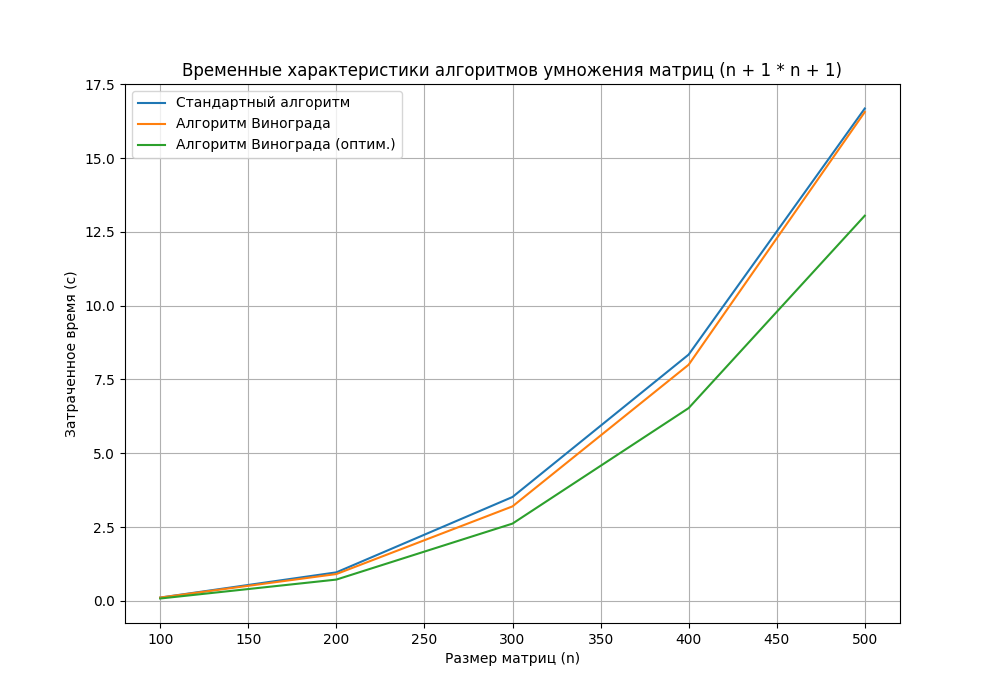
\includegraphics[scale=0.7]{inc/Figure_1.png}}
	
	\caption{Сравнение процессорного времени работы реализаций алгоритмов умножения матриц на квадратных матрицах нечетной размерности (n + 1) * (n + 1)}
	
	\label{fig:fig2}
	
\end{figure}

\clearpage

\section{Оценка затрат алгоритмов по памяти}

Пусть первая матрица (A) имеет N строк и M столбцов, вторая матрица (B) имеет M строк и Q столбцов, тогда затраты памяти на рассматриваемые алгоритмы умножения матриц будут следующими.

Стандартный алгоритм умножения матриц:\\
\begin{itemize}
\item входные матрицы -- (N * M + M * Q) * sizeof(int); 
\item результирующая матрица -- (N * Q) * sizeof(int); 
\item размерности матриц -  3 * sizeof(int).
\end{itemize}

Суммарные затраты памяти cтандартного алгоритма умножения матриц:
(N * M + M * Q + N * Q + 3) * sizeof(int) байт.

Алгоритм Винограда умножения матриц:
\begin{itemize}
\item входные матрицы -- (N * M + M * Q) * sizeof(int); 
\item результирующая матрица -- (N * Q) * sizeof(int); 
\item размерности матриц --  3 * sizeof(int);
\item массивы MulH и MulV -- (N + Q) * sizeof(int);
\item вспомогательные переменные (флаг) -- sizeof(int). (только для оптимизированного алгоритма Винограда)
\end{itemize}

Суммарные затраты памяти алгоритма Винограда умножения матриц:
(N * M + M * Q + N * Q + N + Q + 3) * sizeof(int) байт.

Суммарные затраты памяти оптимизированного алгоритма Винограда умножения матриц:
(N * M + M * Q + N * Q + N + Q + 4) * sizeof(int) байт.

\section*{Вывод}

Таким образом, самой эффективной по времени по экспериментальным данным с учетом работы на всех видах матриц является реализация оптимизированного алгоритма Винограда, стандартный алгоритм и алгоритм Винограда без оптимизации практически одинаковы эффективны по времени из-за того, что неоптимизированный алгоритм Винограда содержит большое количество операций. 

Самым эфективным по памяти является стандартный алгоритм умножения матриц, так как в алгоритме Винограда выделяется память под вспомогательные массивы MulH и MulV.
